\documentclass[aspectratio=169,
hyperref={colorlinks,urlcolor=blue}
]{beamer}


%\usetheme{Pittsburgh}
\usetheme{default}
\usepackage{colortbl}%colored tables
%For using helvetica font:
\usepackage[scaled]{helvet}
\usepackage[T1]{fontenc}
\renewcommand\familydefault{\sfdefault}
\urlstyle{same} %sets the fonts for urls
\usepackage{pdfpages}
\usepackage{siunitx}
\usepackage{caption}
\usepackage{pifont}%for dings
\usepackage{pgfplots}%for 3d plotting
\pgfplotsset{compat = newest}
\usepackage{mathtools}%box in align env \Aboxed
\usepackage[american,smartlabels]{circuitikz}%for drawing circuits
\usepackage{multimedia}
\usepackage{animate}
\usepackage{xcolor}


\usetikzlibrary{arrows}
\usetikzlibrary {3d} 
\usetikzlibrary{decorations.markings, math}
\usetikzlibrary{intersections, pgfplots.fillbetween}
\usetikzlibrary {shapes.geometric} 


%\definecolor{myblue}{RGB}{5, 34, 150}
\definecolor{myblue2}{RGB}{5, 34, 150}
\definecolor{myblue}{RGB}{0,36,82}
\definecolor{myred}{RGB}{207, 2, 13}
\definecolor{mygreen}{RGB}{0, 158, 11}
\definecolor{myyellow}{RGB}{220,220,0}
\definecolor{qblue}{RGB}{0,36,82}
\definecolor{qgold}{RGB}{250,189,15}
\definecolor{qred}{RGB}{185,14,49}
\definecolor{cblue}{rgb}{0.13, 0.67, 0.8}
\definecolor{corange}{rgb}{0.8, 0.34, 0.0}
\definecolor{cpurple}{rgb}{0.54, 0.29, 0.42}

%%%%%%%%%%%% General settings
\setbeamercolor{frametitle}{fg=black}
\setbeamercolor{title}{fg=black}
\setbeamercolor{author}{fg=myblue2}

\beamertemplatenavigationsymbolsempty %no navigation controls at bottom of slides
%\setbeamertemplate{footline}[frame number]
\usefonttheme{professionalfonts} 
\setbeamerfont{title}{series=\bfseries,parent=structure}
\setbeamerfont{frametitle}{series=\bfseries,parent=structure}

%%%%%%%%%%%%Lists
\setbeamertemplate{itemize item}[circle] %{\color{myblue}$\circ$}
\setbeamertemplate{itemize subitem}{\color{myblue2}$\circ$}
\setbeamertemplate{itemize subsubitem}{\color{myblue2}$\cdot$}
\setbeamercolor{itemize item}{bg=myblue2,fg=myblue2}
\setbeamercolor{enumerate item}{bg=myblue2,fg=myblue2}
%%%%%%%%%%%%%%%%%%%%%%%%%%%%

%%%%%%%%%%%%Blocks
\setbeamertemplate{blocks}[rounded]
%Default block
\setbeamercolor{block title}{bg=myblue2, fg=white}
\setbeamercolor{block body}{bg=myblue2!10}
\setbeamerfont{block body}{size=\scriptsize}
\setbeamerfont{block title}{size=\scriptsize}
%Alert block
\setbeamercolor{block title alerted}{bg= myblue2, fg=white}
\setbeamercolor{block body alerted}{bg=myblue2!10}
\setbeamerfont{block body alerted}{size=\scriptsize}
\setbeamerfont{block title alerted}{size=\scriptsize}
%example block
\setbeamercolor{block title example}{bg=mygreen, fg=white}
\setbeamercolor{block body example}{bg=mygreen!10}
\setbeamerfont{block body example}{size=\scriptsize}
\setbeamerfont{block title example}{size=\scriptsize}
%%%%%%%%%%%%%%%%55


%%%%%%%%%%%%Figures and captions
\captionsetup{font=scriptsize,labelfont=scriptsize}
%\setbeamertemplate{caption}{\raggedright\insertcaption\par}
\newenvironment{capfig}[3]{\begin{figure}\includegraphics[width=#1\textwidth]{#2}\caption*{\textit{#3}}\end{figure}}{}

%\makeatother
%\setbeamertemplate{footline}
%{
%  \leavevmode%
%  \hbox{%
%  \begin{beamercolorbox}[wd=.4\paperwidth,ht=2.25ex,dp=1ex,center]{author in head/foot}%
%    \usebeamerfont{author in head/foot}\insertshortauthor
%  \end{beamercolorbox}%
%  \begin{beamercolorbox}[wd=.6\paperwidth,ht=2.25ex,dp=1ex,center]{title in head/foot}%
%    \usebeamerfont{title in head/foot}\insertshorttitle\hspace*{3em}
%    \insertframenumber{} / \inserttotalframenumber\hspace*{1ex}
%  \end{beamercolorbox}
%  }%
%  \vskip0pt%
%}
%\makeatletter

\makeatother
\setbeamertemplate{footline}
{
  \leavevmode%
  \hbox{%
\begin{beamercolorbox}[wd=.27\paperwidth,ht=2.25ex,dp=1ex,center]{author in head/foot}%
    \color{black}{\insertinstitute}
\end{beamercolorbox}
  \begin{beamercolorbox}[wd=.27\paperwidth,ht=2.25ex,dp=1ex,center]{author in head/foot}%
    \color{black}{\inserttitle}
  \end{beamercolorbox}%
  \begin{beamercolorbox}[wd=.27\paperwidth,ht=2.25ex,dp=1ex,center]{title in head/foot}%
    \color{black}{\insertshortauthor}
  \end{beamercolorbox}
  \begin{beamercolorbox}[wd=.27\paperwidth,ht=2.25ex,dp=1ex,center]{title in head/foot}%
    \hspace{.28\paperwidth}\color{black} \insertframenumber{} / \inserttotalframenumber\hspace*{1ex}
  \end{beamercolorbox}
  }%
  \vskip0pt%
}
\makeatletter

\setbeamertemplate{title page}
{
  \begin{tikzpicture}[remember picture,overlay]
    \def\barh{4}%15
  
    \draw[color=myblue2,line width=\barh] ([yshift=-0.5*\barh]current page.north west) -- ([yshift=-0.5*\barh,xshift=-0.67\paperwidth]current page.north east);
    \draw[color=myblue2,line width=\barh] ([yshift=-0.5*\barh,xshift=-0.67\paperwidth]current page.north east) -- ([yshift=-0.5*\barh,xshift=-0.34\paperwidth]current page.north east);
    \draw[color=myblue2,line width=\barh] ([yshift=-0.5*\barh,xshift=-0.34\paperwidth]current page.north east) -- ([yshift=-0.5*\barh]current page.north east); 
  
    \draw[color=myblue2,line width=\barh] ([yshift=0.5*\barh]current page.south west) -- ([yshift=0.5*\barh,xshift=-0.67\paperwidth]current page.south east);
    \draw[color=myblue2,line width=\barh] ([yshift=0.5*\barh,xshift=-0.67\paperwidth]current page.south east) -- ([yshift=0.5*\barh,xshift=-0.34\paperwidth]current page.south east);
    \draw[color=myblue2,line width=\barh] ([yshift=0.5*\barh,xshift=-0.34\paperwidth]current page.south east) -- ([yshift=0.5*\barh]current page.south east);
    %\node[left] at (current page.east) {
    %
\includegraphics[scale=0.1]{figures/coverpage}
    %};
  \end{tikzpicture}
  
  \usebeamerfont{title}\usebeamercolor[fg]{title}\inserttitle\par
  \usebeamerfont{subtitle}\usebeamercolor[fg]{subtitle}\insertsubtitle\par
  \vspace{2cm}
  \usebeamerfont{author}\usebeamercolor[fg]{author}\insertauthor\par
  \usebeamerfont{institute}\usebeamercolor[fg]{author}\insertinstitute\par
  \usebeamercolor[fg]{author}\par
  \usebeamercolor[fg]{titlegraphic}\inserttitlegraphic

} 

\setbeamertemplate{frametitle}{%
    \nointerlineskip%
        \par\hspace*{-\dimexpr0.5\paperwidth-0.5\textwidth}\textcolor{myblue2}{\rule{0.33\paperwidth}{6pt}}\textcolor{myblue2}{\rule{0.33\paperwidth}{6pt}}\textcolor{myblue2}{\rule{0.34\paperwidth}{6pt}} 
    \begin{beamercolorbox}[wd=\paperwidth,ht=0.75cm,dp=0.6ex]{frametitle}
        \hspace*{0.5cm}\strut\usebeamerfont{frametitle}\insertframetitle\strut
        %\hrule
    \end{beamercolorbox}%
    %%Line below:
%\par\hspace*{-\dimexpr0.5\paperwidth-0.5\textwidth}\textcolor{myblue}{\rule{\paperwidth}{0.4pt}}
     % <-- calculation of left margin width + rule
     %\textcolor{red}{\noindent\rule{\paperwidth}{2pt}}
}


%%%%%%%%%%%%Frame templates

%Slide with title
\newenvironment{titleframe}[1]
{\begin{frame}\frametitle{#1}\end{frame}}
{}

%Slide with title and itemize list:
\newenvironment{bulletframe}[1]
{\begin{frame}{#1} \itemize}
{\enditemize \end{frame}}

%Slide with two columns 50/50
\newenvironment{twocolframe}[3]
{\begin{frame}{#1}
 \begin{columns}[T]
 \column{0.5\textwidth}#2
 \column{0.5\textwidth}#3
 \end{columns}\end{frame}}{}

%Slide with two columns 60/40 <<<<<<<<<<<<<<<<<<<<<<  This one!
\newenvironment{twocolframesf}[3]
{\begin{frame}{#1}
 \begin{columns}[T]
 \column{0.6\textwidth}#2
 \column{0.4\textwidth}#3
 \end{columns}\end{frame}}{}
 
%Slide with two columns 70/30
\newenvironment{twocolframest}[3]
{\begin{frame}{#1}
 \begin{columns}[T] 
 \column{0.7\textwidth}#2
 \column{0.3\textwidth}#3
 \end{columns}\end{frame}}{} 
 
%Slide with two columns 40/60
\newenvironment{twocolframefs}[3]
{\begin{frame}{#1}
 \begin{columns}[T] 
 \column{0.4\textwidth}#2
 \column{0.6\textwidth}#3
 \end{columns}\end{frame}}{}
 
%Slide with two columns 70/30
\newenvironment{twocolframets}[3]
{\begin{frame}{#1}
 \begin{columns}[T] 
 \column{0.3\textwidth}#2
 \column{0.7\textwidth}#3
 \end{columns}\end{frame}}{} 

 
%Colloquium speaker (title, abstract, picture file, speaker name)
\newenvironment{colloquium}[5]
{
\begin{frame}{Colloquium: Friday 1:30pm in Stirling A}
\begin{columns}[T] 
 \column{0.8\textwidth}
 \textbf{#1}\\
 #2
 \column{0.2\textwidth}
 \capfig{#3}{#4}{#5}
 \end{columns}
\end{frame}
}
{} 

%%%%%%%%%%%%%Set Hyperref colors


\hypersetup{
  colorlinks=true,
  linkcolor=blue,    
  urlcolor=blue,     
  citecolor=blue      
}
%%%%%%%%%%%%%TOC bolding
\setbeamerfont{section in toc}{series=\bfseries}



%Frames:
% \twocolframesf 60/40 (fs, st, ts) 
% \titleframe
% bulletframe


%%%%%%%%%%%%%%%%%%%%%%%%%
%%%%%% START OF PRESENTATION %%%%%%
%%%%%%%%%%%%%%%%%%%%%%%%%
\title{Kinematics}
\subject{1D, nD and Circular Motion}
\subtitle{Building Models to Describe our World}


%%%%%%%%%%%%%%%%%%%%%%%%%%%%%%
%%%%%%%%%%%%%%%%%%%%%



\begin{document}

%%%%%%%%%%%%%%%%%%%%%%%%%
%%%%%% Title slide %%%%%%
%%%%%%%%%%%%%%%%%%%%%%%%%
\chaptertitle{Kinematics}
\begin{frame}
\titlepage
\thispagestyle{empty}

\begin{textblock*}{5cm}(11cm,4cm)
    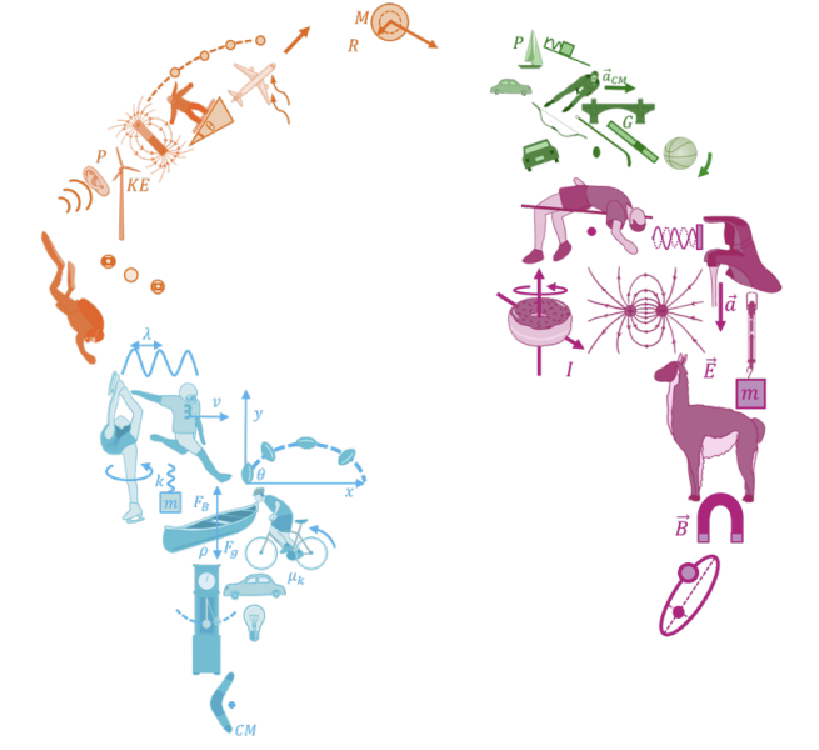
\includegraphics[width=4cm]{figures/BMDW/logo}
\end{textblock*}

\end{frame}

%%%%%%%%%%%%%TOC
\twocolframe{Outline}
  {\tableofcontents[sections={1}, subsectionstyle=show/show]\thispagestyle{empty}}
  {\tableofcontents[sections={2,3}, subsectionstyle=show/show]}
%%%%%%%%%%%%%%%%%%%%%%%%%







%%%%%%%%%%%%%%%%%%%%%%%%%%%%%%%%
\section{1D Kinematics}
\label{sec:1dkinematics}
\title{Kinematics in One Dimension}


%%%%%%%%%%%%%%%%%%%%%%%%%
\begin{frame}
\titlepage
\thispagestyle{empty}
\end{frame}

%


%%%%%%%%%%%%%%%%%%%%%%%%%%%%%%%%
\subsection{Velocity and speed basics}
\label{subsec:velocityandspeedbasics}
\twocolframesf{Average vs instantaneous velocity/speed}
{
\begin{itemize}
\item Velocity is a measure of the rate of change of position.
\item Velocity is positive(negative) if position is increasing(decreasing).
\item Speed is the magnitude of velocity.
\item \textbf{Average velocity}:
\begin{align*}
v=\frac{\Delta x}{\Delta t}
\end{align*}
\item<2-> \textbf{Instantaneous velocity} at some point in time:
\begin{align*}
v=\lim_{\Delta t \to 0}\frac{\Delta x}{\Delta t}=\frac{dx}{dt}
\end{align*}
\end{itemize}
}
{
\centering
\begin{tikzpicture}[%
%https://tex.stackexchange.com/questions/25928/how-to-draw-tangent-line-of-an-arbitrary-point-on-a-path-in-tikz
        tangent/.style={
        decoration={
            markings,% switch on markings
            mark=
                at position ####1
                with
                {
                    \coordinate (tangent point-\pgfkeysvalueof{/pgf/decoration/mark info/sequence number}) at (0pt,0pt);
                    \coordinate (tangent unit vector-\pgfkeysvalueof{/pgf/decoration/mark info/sequence number}) at (1,0pt);
                    \coordinate (tangent orthogonal unit vector-\pgfkeysvalueof{/pgf/decoration/mark info/sequence number}) at (0pt,1);
                }
        },
        postaction=decorate
    },
    use tangent/.style={
        shift=(tangent point-####1),
        x=(tangent unit vector-####1),
        y=(tangent orthogonal unit vector-####1)
    },
    use tangent/.default=1
    ]

\scalebox{1.0}{

 \coordinate (P1) at (0,0.5);
 \coordinate (P2) at (1.75,2); %used to make the path squiggly
 \coordinate (P3) at (3.75,2.5);
 \coordinate (P3x) at ($(0,0)!(P3)!(1,0)$);
 \coordinate (P1P3) at ($(P3)!(P1)!(P3x)$);
 
 \draw[-latex, line width=1.25pt] (0,0) -- (4.5,0) node[below]{$t$}; 
 \draw[-latex, line width=1.25pt] node[below]{\SI{0}{min}} (0,0) -- (0,3) node[left]{$x$}; 
 
 \fill (P1) circle(2pt);
 \fill (P3) circle(2pt);
 
 %The path with tangent coordinates calculated
 \draw[tangent=0.1,tangent=0.4, line width=1pt] (P1) to [out=10,in=190] (P2) to [out=10,in=260] (P3);
 
 \node[left] at (P1) {\SI{100}{km}};
 \draw[dashed] (P3) -- ($(0,0)!(P3)!(0,1)$) node[left] {\SI{150}{km}};
 \draw[dashed] (P3) -- (P3x) node[below] {\SI{30}{min}};
 \draw[dashed] (P1) -- (P1P3) ;
 
 \only<1>{
 \draw[latex-latex,color=myred,line width=1.5pt] (P3) -- (P1P3) node[midway,left]{$\Delta x$};
 \draw[latex-latex,color=myred,line width=1.5pt] (P1) -- (P1P3) node[midway,above]{$\Delta t$};
 }
 
 
 \only<2>{
 \draw [myred, line width=1.5, use tangent=1] (-0.5,0) -- (0.5,0) node[right]{$v=\frac{dx}{dt}$};
 \draw [myred, line width=1.5, use tangent=2] (-0.5,0) -- (0.5,0) node[left]{$v=\frac{dx}{dt}$};
 }
 

}
\end{tikzpicture}
\only<1>{
\captionof*{figure}{\textit{Position as a function of time. Average velocity is the total displacement divided by the total time.}}
}
\only<2>{
\captionof*{figure}{\textit{Position as a function of time. Instantaneous velocity is the derivative at any given point.}}
}
}


%%%%%%%%%%%%%%%%%%%%%%%%%%%%%%%%




%%%%%%%%%%%%%%%%%%%%%%%%%%%%%%%
\subsection{Acceleration}
\label{subsec:acceleration}
\begin{bulletframe}{Acceleration}
\item Acceleration is the rate of change of velocity
\item Average acceleration :
\begin{align*}
a=\frac{\Delta v}{\Delta t}
\end{align*}
\item Instantaneous acceleration at some point in time:
\begin{align*}
a(t)&=\lim_{\Delta t \to 0}\frac{\Delta v}{\Delta t}=\frac{dv}{dt}\\
\therefore v(t) &= \int a(t) dt
\end{align*}
\end{bulletframe}


%%%%%%%%%%%%%%%%%%%%%%%%%%%%%%%%

\begin{bulletframe}{The kinematic equations for constant acceleration}
\scriptsize
\item<1-> If the acceleration is constant:
\begin{align*}
a(t) &= a\\
\therefore v(t) &= \int adt = at+C
\end{align*}
\item<2-> The constant $C$ can be determined from knowing that, say, at $t=0$, $v=v_0$:
\begin{align*}
v(t=0)&=a(0)+C = v_0\\
\therefore C&=v_0\\
\Aboxed{\therefore v(t)&= v_0 + at}
\end{align*}
\item<3-> Since velocity is the time-derivative of position, $x(t)$, position is the anti-derivative of velocity:
\begin{align*}
x(t)=\int v(t) dt = \int (at+v_0) dt = \frac{1}{2}at^2+v_0 t+C'
\end{align*}
\item<4-> Again, we can determine the second integration constant, $C'=x_0$, if we know that $x =x_0$  at $t=0$:
\begin{align*}
\Aboxed{ x(t) = \frac{1}{2}at^2+v_0 t+x_0}
\end{align*}
\end{bulletframe}


%%%%%%%%%%%%%%%%%%%%%%%%%%%%%%%%
\subsection{Group activity: kinematics scetching}
\label{subsec:grpactivitykinematics}
\twocolframe{Group question}
{
Using the following graph of $a(t)$, sketch out the corresponding $v(t)$ and $x(t)$. \textbf{Assume that, at $t=0$, the position is negative and that the speed is positive.}
}
{


\centering
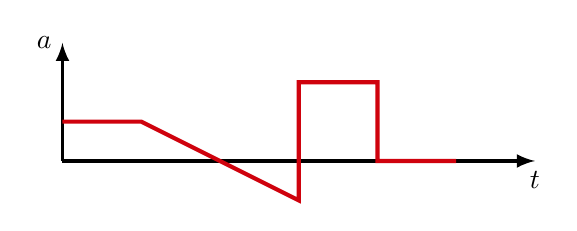
\begin{tikzpicture}[scale =1]

\scalebox{1.0}{

 \coordinate (P1) at (0,0.5);
 \coordinate (P2) at (1,0.5); %used to make the path squiggly
 \coordinate (P3) at (2,0);
 \coordinate (P4) at (3,-0.5);
 \coordinate (P5) at (3,1);
 \coordinate (P6) at (4,1);
 \coordinate (P7) at (4,0);
 \coordinate (P8) at (5,0);
 \coordinate (P1x) at ($(0,0)!(P1)!(1,0)$);
 \coordinate (P2x) at ($(0,0)!(P2)!(1,0)$);
 \coordinate (P3x) at ($(0,0)!(P3)!(1,0)$);
 \coordinate (P4x) at ($(0,0)!(P4)!(1,0)$);
 \coordinate (P5x) at ($(0,0)!(P5)!(1,0)$);
 
 \draw[-latex, line width=1.25pt] (0,0) -- (6,0) node[below]{$t$}; 
 \draw[-latex, line width=1.25pt] (0,0) -- (0,1.5) node[left]{$a$}; 
 
 
 \draw[line width =1.5pt,color=myred] (P1) -- (P2) -- (P3) -- (P4) -- (P5) -- (P6) -- (P7) -- (P8);
 

}
\end{tikzpicture}

\captionof*{figure}{\textit{Acceleration as a function of time.}}

}

%%%%%%%%%%%%%%%%%%%%%%%%%%%%%%%%

\twocolframe{Velocity, $v(t)$}
{
\begin{enumerate}
\item Acceleration is constant and positive, velocity increases linearly.
\item Acceleration is decreasing to zero, velocity increases less and less
\item Acceleration becomes more negative, velocity increases in the negative direction more and more
\item Acceleration is constant and positive, velocity increases linearly.
\item Acceleration is zero, velocity is constant.
\end{enumerate}
}
{

\centering
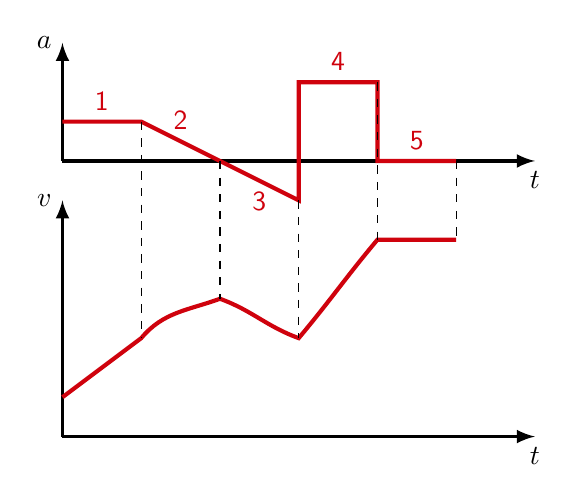
\begin{tikzpicture}[scale =1]
\tikzmath{
\ysh=-3.5;
}

\scalebox{1.0}{

 \coordinate (P1) at (0,0.5);
 \coordinate (P2) at (1,0.5); %used to make the path squiggly
 \coordinate (P3) at (2,0);
 \coordinate (P4) at (3,-0.5);
 \coordinate (P5) at (3,1);
 \coordinate (P6) at (4,1);
 \coordinate (P7) at (4,0);
 \coordinate (P8) at (5,0);
 \coordinate (P1x) at ($(0,0)!(P1)!(1,0)$);
 \coordinate (P2x) at ($(0,0)!(P2)!(1,0)$);
 \coordinate (P3x) at ($(0,0)!(P3)!(1,0)$);
 \coordinate (P4x) at ($(0,0)!(P4)!(1,0)$);
 \coordinate (P5x) at ($(0,0)!(P5)!(1,0)$);
 
 %a
 \draw[-latex, line width=1.25pt] (0,0) -- (6,0) node[below]{$t$}; 
 \draw[-latex, line width=1.25pt] (0,0) -- (0,1.5) node[left]{$a$}; 
 
 \draw[line width =1.5pt,color=myred] (P1) -- (P2) node[midway,above]{1} -- (P3)  node[midway,above]{2}-- (P4) node[midway,below]{3} -- (P5)  -- (P6)  node[midway,above]{4}-- (P7)  -- (P8) node[midway,above]{5};
 
 %vaxis
 \draw[-latex, line width=1.25pt] (0,\ysh) -- (6,\ysh) node[below]{$t$}; 
 \draw[-latex, line width=1.25pt] (0,\ysh) -- (0,\ysh+3) node[left]{$v$}; 
 
 \coordinate (P1V) at (0,\ysh+0.5);
 \coordinate (P2V) at (1,\ysh+1.25);
 \coordinate (P3V) at (2,\ysh+1.75);
 \coordinate (P4V) at (3,\ysh+1.25);
 \coordinate (P5V) at (3,\ysh+0.5);
 \coordinate (P6V) at (4,\ysh+2.5);
 \coordinate (P7V) at (4,\ysh+0.5);
 \coordinate (P8V) at (5,\ysh+2.5);
 
 \draw[line width =1.5pt,color=myred] (P1V) to (P2V) [out=50,in=200] to (P3V) [out=340,in=160] to (P4V) [out=50,in=230]  to (P6V) [out=0,in=180] to (P8V) ;

 \draw[dashed] (P2) -- (P2V);
 \draw[dashed] (P3) -- (P3V);
 \draw[dashed] (P4) -- (P4V);
 \draw[dashed] (P6) -- (P6V);
 \draw[dashed] (P8) -- (P8V);
 
}
\end{tikzpicture}

\captionof*{figure}{\textit{Velocity from acceleration, the object always goes in the positive direction}}

}

%%%%%%%%%%%%%%%%%%%%%%%%%%%%%%%%

\twocolframe{Position, $x(t)$}
{
\begin{enumerate}
\item Velocity increases linearly, position increase quadratically
\item Velocity increases less and less, position increases less than quadratically
\item Positive velocity decreases, position decreases less than quadratically.
\item Velocity increases linearly, position increase quadratically
\item Velocity is constant, position increases linearly
\end{enumerate}
}
{

\centering
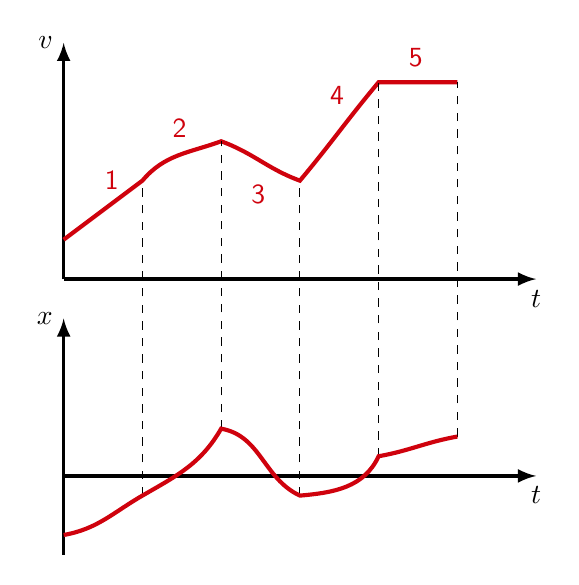
\begin{tikzpicture}[scale =1]
\tikzmath{
\ysh=0;
\xsh=-2.5;
}

\scalebox{1.0}{

 
 %vaxis
 \draw[-latex, line width=1.25pt] (0,\ysh) -- (6,\ysh) node[below]{$t$}; 
 \draw[-latex, line width=1.25pt] (0,\ysh) -- (0,\ysh+3) node[left]{$v$}; 
 
 \coordinate (P1V) at (0,\ysh+0.5);
 \coordinate (P2V) at (1,\ysh+1.25);
 \coordinate (P3V) at (2,\ysh+1.75);
 \coordinate (P4V) at (3,\ysh+1.25);
 %\coordinate (P5V) at (3,\ysh+0.5);
 \coordinate (P6V) at (4,\ysh+2.5);
 %\coordinate (P7V) at (4,\ysh+0.5);
 \coordinate (P8V) at (5,\ysh+2.5);
 
 \draw[line width =1.5pt,color=myred] (P1V) to (P2V) [out=50,in=200] to (P3V) [out=340,in=160] to (P4V) [out=50,in=230]  to (P6V) [out=0,in=180] to (P8V) ;

 %xaxis
 \draw[-latex, line width=1.25pt] (0,\xsh) -- (6,\xsh) node[below]{$t$}; 
 \draw[-latex, line width=1.25pt] (0,\xsh-1) -- (0,\xsh+2) node[left]{$x$}; 


 \coordinate (P1X) at (0,\xsh-0.75);
 \coordinate (P2X) at (1,\xsh-0.25);
 \coordinate (P3X) at (2,\xsh-0.+0.6);
 \coordinate (P4X) at (3,\xsh-0.25);
 \coordinate (P6X) at (4,\xsh+0.25);
 \coordinate (P8X) at (5,\xsh+0.5);

 \draw[dashed] (P2X) -- (P2V);
 \draw[dashed] (P3X) -- (P3V);
 \draw[dashed] (P4X) -- (P4V);
 \draw[dashed] (P6X) -- (P6V);
 \draw[dashed] (P8X) -- (P8V);
 
 \draw[line width =1.5pt,color=myred] (P1X) to [out=10,in=210] (P2X) to [out=30, in=240] (P3X) to [out=-10, in=155] (P4X) to [out=5, in=245] (P6X) to [out=10, in=190] (P8X);
 
 \node[left=5pt,color=myred] at (P2V) {1};
 \node[left=15pt,above=-2pt,color=myred] at (P3V) {2};
 \node[left=15pt,below=-2pt,color=myred] at (P4V) {3};
 \node[left=15pt,below=-2pt,color=myred] at (P6V) {4};
 \node[left=15pt,above=2pt,color=myred] at (P8V) {5};
 
% 
}
\end{tikzpicture}

\captionof*{figure}{\textit{Position from velocity}}

,}
%%%%%%%%%%%%%%%%%%%%%%%%%%%%

\subsection{Relative motion notation in 1D}
\label{subsec:relmotionnotation1d}
\twocolframest{1D Relative motion - notation}
{
\begin{itemize}
\item We can think of different ``frames of reference'', i.e. different coordinate systems that move relative to each other
\item We choose to use primes (‘) to denote quantities in one frame of reference, and letters to identify the object:
\begin{align*}
\textcolor{myred}{v^{'A}}=\textcolor{myblue}{v^{'B}}+v^A
\end{align*}
\end{itemize}


In words:\textcolor{myred}{The velocity of Alice as measured in the prime reference frame (Igor, the ground)} \textcolor{myblue}{is the velocity of Brice (the train) measured relative to the ground} plus \textbf{the velocity of Alice measured relative to the un-primed reference frame} (aka Brice).
}
{
\capfig{1}{figures/Kinematics/trainABC}{Igor watches a train with Brice (sitting) and Alice (walking) in it.}
Same idea with position:
\begin{align*}
\textcolor{myred}{x^{'A}}&=\textcolor{myblue}{x^{'B}}+x^A\\
\textcolor{myred}{x^{'A}}&=\textcolor{myblue}{v^{'B}t}+x^A
\end{align*}
}





%%%%%%%%%%%%%%%%%%%%%%%%%%%%


\section{nD Kinematics}
\label{sec:ndkinematics}
\title{Kinematics in Multiple Dimensions}
\institute{Mathmatical Tools and Their Use In Physics}
\author{\insertsubsection}


%%%%%%%%%%%%%%%%%%%%%%%%%
\begin{frame}
\titlepage
\thispagestyle{empty}
\end{frame}
%%%%%%%%%%%%%%%%%%%%%%%%%%















%%%%%%%%%%%%%%%%%%%%%%%%%%%%%
\subsection{2D motion}
\label{subsec:2dmotion}
\begin{bulletframe}{2D motion}
\item Same as 1D, but we need to describe both of the x and y coordinates of the object
\item The most compact notation to do this is to use vectors
\item Position:
\begin{align*}
\vec r (t) = \begin{pmatrix}
x(t)\\y(t)
\end{pmatrix}
\end{align*}
By specifying the vector,$\vec r (t)$ , relative to the origin of an $xy$ coordinate system, we fully specify the position of an object (namely its $x$ and $y$ coordinates as a function of time.
\end{bulletframe}



%%%%%%%%%%%%%%%%%%%%%%%%%%%%%%%%
\subsection{Relative motion notation in 2D}
\label{subsec:relmotionnotation2d}
\twocolframest{2D Relative motion - notation}
{
\begin{itemize}
\item We can think of different ``frames of reference'', i.e. different coordinate systems that move relative to each other
\item We choose to use primes (‘) to denote quantities in one frame of reference, and letters to identify the object:
\begin{align*}
\textcolor{myred}{\vec v^{'A}}=\textcolor{myblue}{\vec v^{'B}}+\vec v^A
\end{align*}
\end{itemize}


In words:\textcolor{myred}{The velocity of Alice as measured in the prime reference frame (Igor, the ground)} \textcolor{myblue}{is the velocity of Brice (the train) measured relative to the ground} plus \textbf{the velocity of Alice measured relative to the un-primed reference frame} (aka Brice).
}
{
\capfig{1}{figures/Kinematics/trainABC}{Igor watches a train with Brice (sitting) and Alice (walking) in it.}
Same idea with position:
\begin{align*}
\textcolor{myred}{\vec r^{'A}}&=\textcolor{myblue}{\vec r^{'B}}+\vec r^A\\
\textcolor{myred}{\vec r^{'A}}&=\textcolor{myblue}{\vec v^{'B}t}+\vec r^A
\end{align*}
}



%%%%%%%%%%%%%%%%%%%%%%%%%%%%%%%%


%%%%%%%%%%%%%%%%%%%%%%%%%%%%%%%%
\subsection{Building a model: feed the monkey!}
\label{subsec:buildingmodelmonkey}
\twocolframesf{Feeding the monkey: building a model}
{
$\rightarrow$ How do we throw the banana in order for the monkey to catch it? The monkey will let go of the branch as soon as we throw the banana.
}
{
\capfig{1}{figures/Kinematics/MonkeyTreeExample}{As soon as the banana is released, the monkey lets go of the branch. How to throw the banana for the monkey to catch it?}
}


%%%%%%%%%%%%%%%%%%%%%%%%%%%%%%%%
\twocolframesf{Start with initial conditions}
{
\begin{itemize}
\item We choose a coordinate system $\rightarrow$ in this case: origin at starting position of banana, $y$ positive up, $x$ positive right
\item We have 2 objects, the banana and the monkey, whose motion we want to describe:
\begin{align*}
\vec r_b(t), \vec r_m(t)
\end{align*}
\item At time $t=0$, they have initial position and velocity vectors:
\begin{align*}
\vec r_{b0}, \vec r_{m0}, \textcolor{myred}{\vec v_{b0}}, \vec v_{m0}
\end{align*}
\item We want to determine $\textcolor{myred}{\vec v_{b0}}$, the initial velocity of the banana
\end{itemize}
}
{
\capfig{1}{figures/Kinematics/MonkeyTreeExample}{As soon as the banana is released, the monkey lets go of the branch. How to throw the banana for the monkey to catch it?}
\begin{tikzpicture}[remember picture,overlay]%
 \draw[-latex, line width=2, color=myred] ($(current page.center)+(2.3,-0.55)$) -- +(1.5,0.625) node[above]{$\vec v_{b0}$} ;%
 \draw[line width =1.5, color=myred] ($(current page.center)+(3.1,-0.55)$) arc (0:22.6:0.8) node[midway,right] {$\theta$};
\end{tikzpicture}
}


%%%%%%%%%%%%%%%%%%%%%%%%%%%%%%%%




%%%%%%%%%%%%%%%%%%%%%%%%%%%%%%%%
\twocolframesf{Equate the positions of the banana and monkey}
{\scriptsize
\begin{itemize}
\item For constant acceleration:
\begin{align*}
\vec r(t) = \vec r_0 + \vec v_0 t + \frac{1}{2} \vec a t^2
\end{align*}
\item<2-> For the banana, $\vec r_{b0}=0$, this gives:
\begin{align*}
\vec r_b (t) = v_{b0} \begin{pmatrix}
\cos\theta \\ \sin\theta
\end{pmatrix}
t+ \frac{1}{2} \begin{pmatrix}
0\\ \SI{-9.8}{m/s^2}
\end{pmatrix}t^2
\end{align*}
\item<3-> For the monkey, $\vec v_{m0}=0$, this gives:
\begin{align*}
\vec r_m (t) = \begin{pmatrix}
d \\ h
\end{pmatrix}
+ \frac{1}{2} \begin{pmatrix}
0\\ \SI{-9.8}{m/s^2}
\end{pmatrix}t^2
\end{align*}

\end{itemize}
}
{\scriptsize
\begin{itemize}
\item<4-> The positions must be the same at some time $t$, $\vec r_b (t)=\vec r_m (t)$, writing this out for each component:
\begin{align*}
v_{b0}\cos\theta t&= d\\
v_{b0}\sin\theta t-\frac{1}{2}(\SI{9.8}{m/s^2}) t^2&= h-\frac{1}{2}(\SI{9.8}{m/s^2})t^2
\end{align*}
\item<5-> Simplify:
\begin{align*}
v_{b0}\cos\theta t&= d\\
v_{b0}\sin\theta t&= h
\end{align*}
\item<6> Divide one equation by the other to eliminate $t, v_{b0}$ and get $\theta$:
\begin{align*}
\frac{\sin\theta}{\cos \theta}=\Aboxed{\tan\theta=\frac{h}{d}}
\end{align*}
\end{itemize}
}

%%%%%%%%%%%%%%%%%%%%%%%%%%%%%%%%
\twocolframesf{Thinking about the model, $\tan\theta=\frac{h}{d}$}
{
\begin{itemize}
\item This is somewhat surprising; all we have to do is aim for the monkey...
\item The speed at which we throw the banana does not matter!
\item If we throw the banana faster, it will intercept the monkey higher above the ground.
\item Think of this in the absence of gravity (then you obviously aim for the monkey) – in the presence of gravity, both the banana and monkey move downwards by the same amount in the same amount of time, $\textcolor{myred}{\frac{1}{2}gt^2}$
\end{itemize}
}
{
\capfig{1}{figures/Kinematics/MonkeyTreeExample}{As soon as the banana is released, the monkey lets go of the branch. How to throw the banana for the monkey to catch it? Just aim for the monkey!}
\begin{tikzpicture}[remember picture,overlay]%
 \draw[-latex, line width=2, color=myred] ($(current page.center)+(2.3,-0.55)$) -- +(1.5,0.625) node[above]{$\vec v_{b0}$} ;%
 \draw[line width=0.75, dashed, color=myred] ($(current page.center)+(2.3,-0.55)$) -- +(3,1.25) ;%
 \draw[line width =1.5, color=myred] ($(current page.center)+(3.1,-0.55)$) arc (0:22.6:0.8) node[midway,right] {$\theta$};
\end{tikzpicture}
}
%%%%%%%%%%%%%%%%%%%%%%%%%%%%%%%%%%%%%%%5

\subsection{Zeno's paradox}
\label{subsec:zenosparadox}
\begin{frame}{Zeno's paradox}
An example of Zeno's paradox: If you shoot an arrow at speed, $v$, towards a target a distance, $D$, away, it must first cover half the distance. After that, it must still go the other half, so it travels half of that remaining distance. If you think of it this way, like Zeno, you appear to have a different paradox, the arrow can never get there because there is always a small distance left. Any motion is thus impossible!

\end{frame}

\twocolframesf{Zeno's arrow: Kinematics to the rescue!}
{
\begin{itemize}
\item At constant speed, $v$, it will take a time, $T$, for the arrow to cover the distance, $D$:
\begin{align*}
T=\frac{D}{v}
\end{align*}
\item The time that it will take to cover the first, second, third segments:
\begin{align*}
t_1=\frac{D}{2v}\quad t_2=\frac{D}{4v}\quad t_3=\frac{D}{8v}\;\; \dots \;\; t_N=\frac{D}{2vN}
\end{align*}
\item The total time is thus also given by:
\begin{align*}
T=t_1+t_2+t_3+\dots=\sum_{i=1}^N t_i=\frac{D}{v}\sum_{1=1}^N\frac{1}{2i}
\end{align*}

\end{itemize}
}
{
\vspace{-1.5cm}
\begin{center}
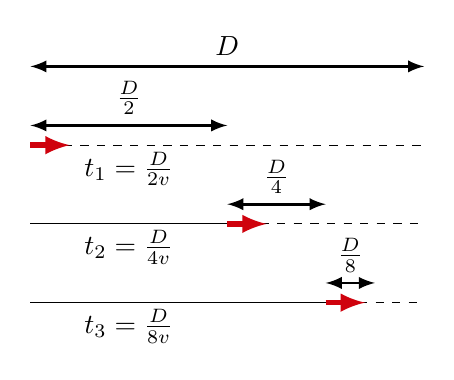
\begin{tikzpicture}[scale=1]
\tikzmath{
\L=5;
\h=1;
\lv=0.5;
}
\scalebox{1.0}{
%\draw[line width=2] (0,0) -- (\L,0);
\draw[latex-latex,line width=1] (0,0) -- (\L,0) node[midway,above]{$D$};
%\fill (0,0) circle (2pt);
%\fill (\L,0) circle (2pt);

\draw[dashed] (0,-\h) -- +(\L,0);
\draw[latex-latex,line width=1] (0,-\h+0.25) -- +(\L/2,0) node[midway,above]{$\frac{D}{2}$};
\draw[-latex,line width=2, color=myred] (0,-\h)--+(\lv,0);
\node at (\L/4,-\h-0.3){$t_1=\frac{D}{2v}$};

\draw[dashed] (\L/2,-2*\h) -- +(\L/2,0);
\draw[latex-latex,line width=1] (\L/2,-2*\h+0.25) -- +(\L/4,0) node[midway,above]{$\frac{D}{4}$};
\draw[](0,-2*\h) -- +(\L/2,0);
\draw[-latex,line width=2, color=myred] (\L/2,-2*\h)--+(\lv,0);
\node at (\L/4,-2*\h-0.3){$t_2=\frac{D}{4v}$};

\draw[dashed] (3*\L/4,-3*\h) -- +(\L/4,0);
\draw[latex-latex,line width=1] (3*\L/4,-3*\h+0.25) -- +(\L/8,0) node[midway,above]{$\frac{D}{8}$};
\draw[](0,-3*\h) -- +(3*\L/4,0);
\draw[-latex,line width=2, color=myred] (3*\L/4,-3*\h)--+(\lv,0);
\node at (\L/4,-3*\h-0.3){$t_3=\frac{D}{8v}$};
}
\end{tikzpicture}
\captionof*{figure}{\textit{An arrow traveling Zeno's way!}}
\end{center}
\vspace{-0.5cm}
\only<2>{
\begin{block}{Resolving the paradox:}
The two ways of calculating, $T$, must be equivalent, thus:
\begin{align*}
\lim_{N\to\infty}\sum_{1=1}^N\frac{1}{2i} = 1
\end{align*}
The geometric series converges!
\end{block}
}
}

%%%%%%%%%%%%%%%%%%%%%%












%%%%%%%%%%%%%%%%%%%%%%%%%%%%%%%%
\section{Circular Motion}
\label{sec:circularmotion}
\title{Circular Motion}
\institute{Mathmatical Tools and Their Use In Physics}
\author{\insertsubsection}


%%%%%%%%%%%%%%%%%%%%%%%%%
\begin{frame}
\titlepage
\thispagestyle{empty}
\end{frame}


%%%%%%%%%%%%%%%%%%%%%%%%%%%%%%%%














%%%%%%%%%%%%%%%%%%%%%%%%%%%%%%%%
\subsection{Acceleration with constant speed}
\label{subsec:accelerationwithconstantspeed}
\twocolframesf{Acceleration vector: constant speed}
{
\begin{itemize}
\item The acceleration vector of an object is non-zero if the velocity vector changes.
\item[$\rightarrow$] The velocity vector can change magnitude, direction,\textit{ or both}!
\item<2> For constant speed, the acceleration vector is perpendicular to the velocity vector, in the limit of $\Delta t\to 0$ (as we'll see). 
\end{itemize}
}
{
\begin{center}
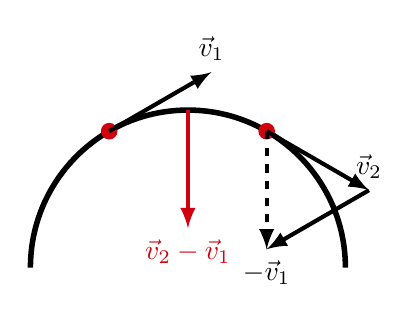
\begin{tikzpicture}[scale=1]
\tikzmath{
\R=2;
\th=30;
\Px=\R*sin(\th);
\Py=\R*cos(\th);
\v=1.5;
\vx=\v*cos(\th);
\vy=\v*sin(\th);
}
\scalebox{1.0}{

\coordinate (P1) at (-\Px,\Py);
\coordinate (P2) at (\Px,\Py);

\draw[line width=2] (\R,0) arc(0:180:\R);
\fill[color=myred] (P1) circle(3pt);
\fill[color=myred] (P2) circle(3pt);

\draw[-latex,line width =1.5] (P1) -- +(\vx,\vy) node[above]{$\vec v_1$};
\draw[-latex,line width =1.5] (P2) -- +(\vx,-\vy) node[above]{$\vec v_2$};

\only<2>{
\draw[-latex,line width =1.5] ($(P2)+(\vx,-\vy)$) -- +(-\vx,-\vy) node[below ]{$-\vec v_1$};
\draw[-latex,dashed,line width =1.5] (P2) -- ($(P2)+(0,-2*\vy)$) ;
\draw[-latex,line width =1.5,color=myred] (0,\R) -- +(0,-2*\vy) node[below] {$\vec v_2-\vec v_1$};
}

}
\end{tikzpicture}
\only<1>{\captionof*{figure}{\textit{Velocity vector of an object going around a circle.}}}
\only<2>{\captionof*{figure}{\textit{The change in velocity vector $ \Delta\vec v=\vec v_2-\vec v_1$ is perpendicular to the trajectory.}}}
\end{center}

}

\subsection{Taking the derivative of a vector}
\label{subsec:takingthederivativeofavector}
%%%%%%%%%%%%%%%%%%%%%%%%%%%%%%%%
\begin{bulletframe}{Taking the derivative of a vector}
\item The average acceleration vector is defined as:
\begin{align*}
\vec a = \frac{\Delta \vec v}{\Delta t}
\end{align*}
\item Dividing a vector by a scalar (divide each component):
\begin{align*}
\begin{pmatrix}
a_x\\a_y
\end{pmatrix}
= \begin{pmatrix}
\frac{\Delta v_x}{\Delta t}\\
\frac{\Delta v_y}{\Delta t}
\end{pmatrix}
\end{align*}
\item The instantaneous acceleration is given by taking $\Delta t \to 0$:
 \begin{align*}
 \vec a = \frac{d}{dt}\vec v=
\begin{pmatrix}
a_x\\a_y
\end{pmatrix}
= \begin{pmatrix}
\frac{d v_x}{dt}\\
\frac{d v_y}{dt}
\end{pmatrix}
\end{align*}
\end{bulletframe}


%%%%%%%%%%%%%%%%%%%%%%%%%%%%%%%%


%%%%%%%%%%%%%%%%%%%%%%%%%%%%%%%%
%%%%%%%%%%%%%%%%%%%%%%%%%%%%%%%%
\subsection{The acceleration vector}
\label{subsec:theaccelerationvector}
\twocolframesf{Acceleration vector: general case}
{
\begin{itemize}
\item In general, the velocity vector can change both magnitude and direction.
\item The acceleration vector, $\vec a$, will, in general, have components that are perpendicular and parallel to the instantaneous velocity:
\begin{itemize}
\item You can think of the \textcolor{myred}{perpendicular component}, $\vec a_\perp$, as being responsible for the \textcolor{myred}{change in direction}.
\item You can think of \textcolor{blue}{the parallel component}, $\vec a_\parallel$, as being responsible for the \textcolor{blue}{change in speed}
\end{itemize}
\end{itemize}
}
{
\begin{center}
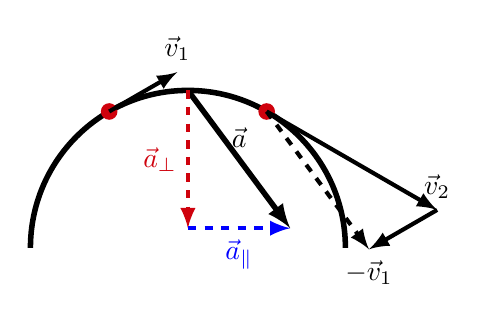
\begin{tikzpicture}[scale=1]
\tikzmath{
\R=2;
\th=30;
\Px=\R*sin(\th);
\Py=\R*cos(\th);
\v=1;
\vx=\v*cos(\th);
\vy=\v*sin(\th);
\vv=2.5;
\vvx=\vv*cos(\th);
\vvy=\vv*sin(\th);
}
\scalebox{1.0}{

\coordinate (P1) at (-\Px,\Py);
\coordinate (P2) at (\Px,\Py);

\draw[line width=2] (\R,0) arc(0:180:\R);
\fill[color=myred] (P1) circle(3pt);
\fill[color=myred] (P2) circle(3pt);

\draw[-latex,line width =1.5] (P1) -- +(\vx,\vy) node[above]{$\vec v_1$};
\draw[-latex,line width =1.5] (P2) -- +(\vvx,-\vvy) node[above]{$\vec v_2$};


\draw[-latex,line width =1.5] ($(P2)+(\vvx,-\vvy)$) -- +(-\vx,-\vy) node[below ]{$-\vec v_1$};
\draw[-latex,dashed,line width =1.5] (P2) -- ($(P2)+(\vvx-\vx,-\vvy-\vy)$) ;
\draw[-latex,line width =2] (0,\R) -- +(\vvx-\vx,-\vvy-\vy) node[midway,above] {$\vec a$};
\draw[-latex,dashed, line width =1.5,color=myred] (0,\R) -- +(0,-\vvy-\vy) node[midway,left] {$\vec a_{\perp}$};
\draw[-latex,dashed, line width =1.5,color=blue] ($(0,\R)+(0,-\vvy-\vy)$) -- +(\vvx-\vx,0) node[midway,below] {$\vec a_{\parallel}$};
}
\end{tikzpicture}
\captionof*{figure}{\textit{The acceleration has a component perpendicular to the trajectory due to the direction changing, and a component parallel due to the magnitude changing.}}
\end{center}

}

%%%%%%%%%%%%%%%%%%%%%%%%%%%

\subsection{Describing motion around a circle}
\label{subsec:describingmotionaroundacircle}
\twocolframesf{Motion along a circle}
{
\begin{itemize}
\item We wish to describe the motion of an object moving along a circular path.
\item This is 2D motion, but constrained along a (1D) line.
\item We have several ways to describe the motion:
\begin{itemize}
\item Using full 2D description, $\vec r(t)$. 
\item Using a 1D description along a curved axis: $s(t)$.
\item Using a 1D description using angular quantities: $\theta(t)$.
\end{itemize}
\item They are, of course, all related and equivalent.
\item 1D is usually more convenient!
\end{itemize}
}
{
\begin{center}
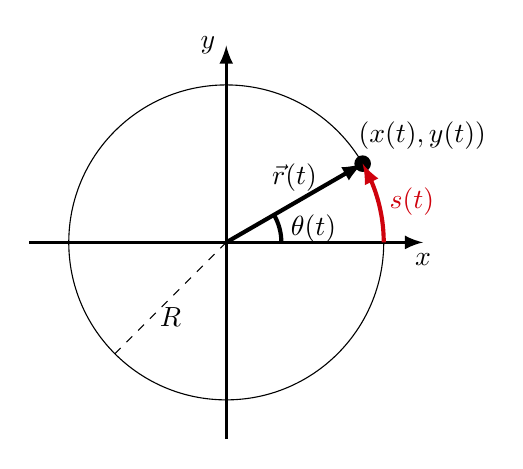
\begin{tikzpicture}[scale=1]
\tikzmath{
\R=2;
\th=30;
\Px=\R*cos(\th);
\Py=\R*sin(\th);
}
\scalebox{1.0}{

\coordinate (P) at (\Px,\Py);

\draw[-latex, line width=1.25pt] (-1.25*\R,0) -- (1.25*\R,0) node[below]{$x$}; 
\draw[-latex, line width=1.25pt] (0,-1.25*\R) -- (0,1.25*\R) node[left]{$y$};

\draw (0,0) circle (\R); 
\fill (P) circle(3pt);
\draw[-latex, line width = 1.5] (0,0) -- (P) node[midway,above] {$\vec r(t)$};
\draw[line width = 1.5] (0.7,0) arc (0:\th:0.7) node[midway,right]{$\theta(t)$};
\draw[-latex, color=myred, line width = 1.5] (\R,0) arc (0:\th:\R) node[midway,right]{$s(t)$};
\node[above=10pt, right=-5pt] at (P) {$\left(x(t),y(t)\right)$};
\draw[dashed] (0,0) --+(225:\R) node[midway,below]{$R$};

}
\end{tikzpicture}
\captionof*{figure}{\textit{Different ways to describe motion around a circle.}}
\end{center}

}


%%%%%%%%%%%%%%%%%%%%%%%%%%%%%%%%

%%%%%%%%%%%%%%%%%%%%%%%%%%%%%%%%
\begin{bulletframe}{Angular velocity and angular acceleration}
\item<1-> The rate of change of the angle (angular velocity):
\begin{align*}
\omega = \frac{d\theta}{dt}
\end{align*}
\item<1-> The rate of change of the angular velocity (angular acceleration)
\begin{align*}
\alpha = \frac{d\omega}{dt}
\end{align*}
\item<2-> For \textbf{constant angular acceleration}, we have (from taking anti-derivatives):
\begin{align*}
\omega(t) &= \omega_0 + \alpha t\\
\theta(t) &= \theta_0+\omega t+\frac{1}{2}\alpha t^2
\end{align*}
If the object was located at $\theta =\theta_0$, with angular velocity, $\omega_0$, at time $t=0$
\end{bulletframe}


%%%%%%%%%%%%%%%%%%%%%%%%%%%%%%%%

%%%%%%%%%%%%%%%%%%%%%%%%%%%%%%%%
\twocolframesf{Relating $\theta(t)$ and $s(t)$}
{\scriptsize
\begin{itemize}
\item The angular position:
\begin{align*}
\theta(t)=\frac{1}{R} s(t)
\end{align*}
\item<2-> The angular velocity:
\begin{align*}
\omega(t)=\frac{d}{dt} \left(\frac{1}{R}s(t)\right)=\frac{1}{R}\frac{ds}{dt}=\frac{1}{R}v_s
\end{align*}
\item<2-> The angular acceleration:
\begin{align*}
\alpha(t)=\frac{d}{dt} \left(\frac{1}{R}v_s(t)\right)=\frac{1}{R}\frac{dv_s}{dt}=\frac{1}{R}a_s
\end{align*}
\item<2-> The ``linear'' or ``tangential'' ($s,v_s,a_s$) and angular ($\theta,\omega,\alpha$) quantities are connected by the radius $R$:
\begin{align*}
\text{linear quantity}=R\times\text{angular quantity}
\end{align*}
\end{itemize}
}
{
\begin{center}
\vspace{-1cm}
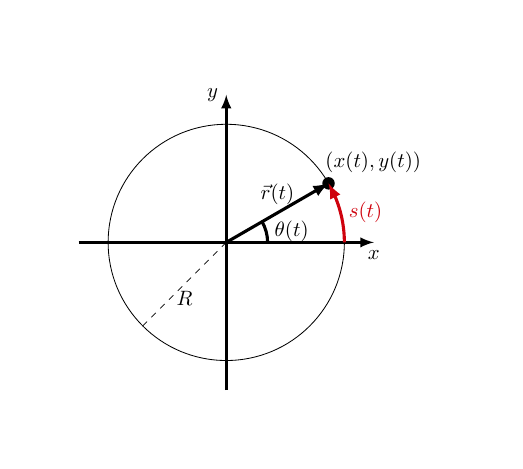
\begin{tikzpicture}[scale=1]
\tikzmath{
\R=2;
\th=30;
\Px=\R*cos(\th);
\Py=\R*sin(\th);
}
\scalebox{0.75}{

\coordinate (P) at (\Px,\Py);

\draw[-latex, line width=1.25pt] (-1.25*\R,0) -- (1.25*\R,0) node[below]{$x$}; 
\draw[-latex, line width=1.25pt] (0,-1.25*\R) -- (0,1.25*\R) node[left]{$y$};

\draw (0,0) circle (\R); 
\fill (P) circle(3pt);
\draw[-latex, line width = 1.5] (0,0) -- (P) node[midway,above] {$\vec r(t)$};
\draw[line width = 1.5] (0.7,0) arc (0:\th:0.7) node[midway,right]{$\theta(t)$};
\draw[-latex, color=myred, line width = 1.5] (\R,0) arc (0:\th:\R) node[midway,right]{$s(t)$};
\node[above=10pt, right=-5pt] at (P) {$\left(x(t),y(t)\right)$};
\draw[dashed] (0,0) --+(225:\R) node[midway,below]{$R$};

}
\end{tikzpicture}
\end{center}
\vspace{-1cm}
\only<2>{
\begin{align*}
\Aboxed{s(t)&=R\theta(t)}\\
\Aboxed{v_s(t)&=R\omega(t)}\\
\Aboxed{a_s(t)&=R\alpha(t)}
\end{align*}
}
}


%%%%%%%%%%%%%%%%%%%%%%%%%%%%%%%%
\twocolframesf{Vector description for circular motion}
{
\begin{itemize}
\item Velocity from position:
\begin{align*}
\vec r &= R \begin{pmatrix}
\cos\left(\theta(t)\right)\\
\sin\left(\theta(t)\right)
\end{pmatrix}\\
\therefore \vec v &= \frac{d}{dt} \vec r=\frac{d}{dt} R \begin{pmatrix}
\cos\left(\theta(t)\right)\\
\sin\left(\theta(t)\right)
\end{pmatrix}\\
&=R \begin{pmatrix}
\frac{d}{dt}\cos\left(\theta(t)\right)\\
\frac{d}{dt}\sin\left(\theta(t)\right)
\end{pmatrix}
=R \begin{pmatrix}
-\sin\left(\theta(t)\right)\frac{d\theta}{dt}\\
\cos\left(\theta(t)\right)\frac{d\theta}{dt}
\end{pmatrix}\\
&=R\omega\begin{pmatrix}
-\sin\left(\theta(t)\right)\\
\cos\left(\theta(t)\right)
\end{pmatrix}
\end{align*}

\end{itemize}
Velocity and position are perpendicular. The velocity is tangent to the circle, as expected. The magnitude of the velocity vector is $v=v_s=\omega R$.
}
{
\begin{center}
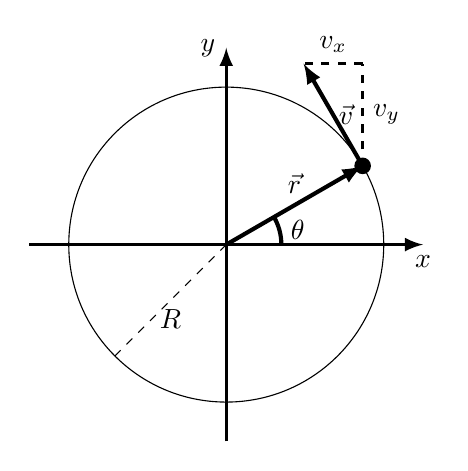
\begin{tikzpicture}[scale=1]
\tikzmath{
\R=2;
\th=30;
\Px=\R*cos(\th);
\Py=\R*sin(\th);
\v=1.5;
\vx=-\v*sin(\th);
\vy=\v*cos(\th);
}
\scalebox{1}{

\coordinate (P) at (\Px,\Py);

\draw[-latex, line width=1.25pt] (-1.25*\R,0) -- (1.25*\R,0) node[below]{$x$}; 
\draw[-latex, line width=1.25pt] (0,-1.25*\R) -- (0,1.25*\R) node[left]{$y$};

\draw (0,0) circle (\R); 
\fill (P) circle(3pt);
\draw[-latex, line width = 1.5] (0,0) -- (P) node[midway,above] {$\vec r$};
\draw[line width = 1.5] (0.7,0) arc (0:\th:0.7) node[midway,right]{$\theta$};
\draw[-latex, line width = 1.5] (P) -- +(\vx,\vy) node[midway,right=-2pt] {$\vec v$};
\draw[dashed, line width = 1.] (P) -- +(0,\vy) node[midway,right] {$v_y$};
\draw[dashed, line width = 1.] ($(P) +(0,\vy)$) -- +(\vx,0) node[midway,above] {$v_x$};

\draw[dashed] (0,0) --+(225:\R) node[midway,below]{$R$};

}
\end{tikzpicture}
\end{center}

}


%%%%%%%%%%%%%%%%%%%%%%%%%%%%%%%%
\twocolframesf{Vector description for circular motion}
{\scriptsize
\begin{itemize}
\item The linear velocity, $v_s$, is the magnitude of the velocity vector:
\begin{align*}
\vec v &= R\omega\begin{pmatrix}
-\sin\left(\theta(t)\right)\\
\cos\left(\theta(t)\right)
\end{pmatrix}=v_s(t)\begin{pmatrix}
-\sin\left(\theta(t)\right)\\
\cos\left(\theta(t)\right)
\end{pmatrix}\\
\therefore ||\vec v||&=v=v_s=R\omega
\end{align*}
\item The direction of the velocity vector is given by:
\begin{align*}
\hat v = \begin{pmatrix}
-\sin\left(\theta(t)\right)\\
\cos\left(\theta(t)\right)
\end{pmatrix}
\end{align*}
which is a unit vector (length of 1).
\item We can write the velocity vector as:
\begin{align*}
\vec v =v(t) \hat v(t)
\end{align*}
\end{itemize}
The direction of the velocity vector, $\hat v$, changes with time, and the magnitude, $v$, could change with time.
}
{
\begin{center}
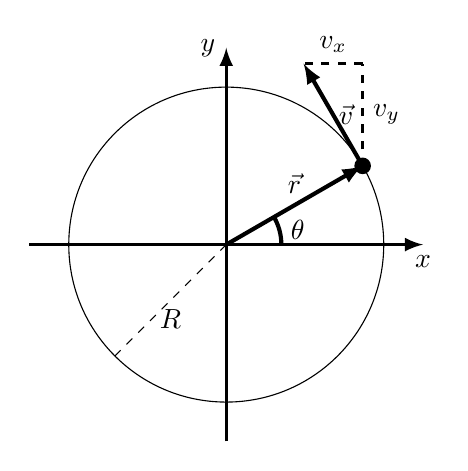
\begin{tikzpicture}[scale=1]
\tikzmath{
\R=2;
\th=30;
\Px=\R*cos(\th);
\Py=\R*sin(\th);
\v=1.5;
\vx=-\v*sin(\th);
\vy=\v*cos(\th);
}
\scalebox{1}{

\coordinate (P) at (\Px,\Py);

\draw[-latex, line width=1.25pt] (-1.25*\R,0) -- (1.25*\R,0) node[below]{$x$}; 
\draw[-latex, line width=1.25pt] (0,-1.25*\R) -- (0,1.25*\R) node[left]{$y$};

\draw (0,0) circle (\R); 
\fill (P) circle(3pt);
\draw[-latex, line width = 1.5] (0,0) -- (P) node[midway,above] {$\vec r$};
\draw[line width = 1.5] (0.7,0) arc (0:\th:0.7) node[midway,right]{$\theta$};
\draw[-latex, line width = 1.5] (P) -- +(\vx,\vy) node[midway,right=-2pt] {$\vec v$};
\draw[dashed, line width = 1.] (P) -- +(0,\vy) node[midway,right] {$v_y$};
\draw[dashed, line width = 1.] ($(P) +(0,\vy)$) -- +(\vx,0) node[midway,above] {$v_x$};

\draw[dashed] (0,0) --+(225:\R) node[midway,below]{$R$};

}
\end{tikzpicture}
\end{center}

}


%%%%%%%%%%%%%%%%%%%%%%%%%%%%%%%%
\subsection{Deriving the acceleration vector}
\label{subsec:deriveaccvector}
\begin{frame}{Acceleration for circular motion}
\begin{itemize}
\item<1-> The acceleration vectors is given by:
\begin{align*}
\vec a = \frac{d}{dt} \vec v = \frac{d}{dt} \textcolor{blue}{v(t)} \textcolor{myred}{\hat v (t)}
\end{align*}
\item<2-> Use the product rule for derivatives:
\begin{align*}
\vec a = \textcolor{blue}{\frac{dv}{dt} \hat v (t)}+ \textcolor{myred}{v(t)\frac{d\hat v}{dt} }
\end{align*}
\item<3-> Part of the acceleration vector is due to \textcolor{blue}{change in speed, $\frac{dv}{dt}$, and is \textbf{parallel} to the velocity, $\hat v$}, and part is due to \textcolor{myred}{change in direction, $\frac{d\hat v}{dt}$ and in a \textbf{different direction}}:
\begin{align*}
\vec a = \textcolor{blue}{a_s \hat v (t)}+ \textcolor{myred}{v(t)\frac{d}{dt} \begin{pmatrix}
-\sin\left(\theta(t)\right)\\
\cos\left(\theta(t)\right)
\end{pmatrix}}
\end{align*}
\end{itemize}

\end{frame}


%%%%%%%%%%%%%%%%%%%%%%%%%%%%%%%%
\begin{frame}{The change in direction}
\begin{itemize}
\item<1-> Apply the Chain Rule (again) to obtain the change in direction:
\begin{align*}
\textcolor{myred}{\frac{d\hat v}{dt}}=
\textcolor{myred}{\frac{d}{dt} \begin{pmatrix}
-\sin\left(\theta(t)\right)\\
\cos\left(\theta(t)\right)
\end{pmatrix}} = \textcolor{myred}{ \begin{pmatrix}
-\cos\left(\theta(t)\right)\frac{d\theta}{dt}\\
-\sin\left(\theta(t)\right)\frac{d\theta}{dt}
\end{pmatrix}} = \textcolor{myred}{\omega \begin{pmatrix}
-\cos\left(\theta(t)\right)\\
-\sin\left(\theta(t)\right)\end{pmatrix}}
\end{align*}
\item<2-> Note that this is perpendicular to the velocity ($\hat v$) and has magnitude of $\omega$. The vector $\textcolor{myred}{\frac{d\hat v}{dt}}$ points towards the centre of the circle.
\end{itemize}
\only<2>{
\vspace{-0.75cm}
\begin{center}
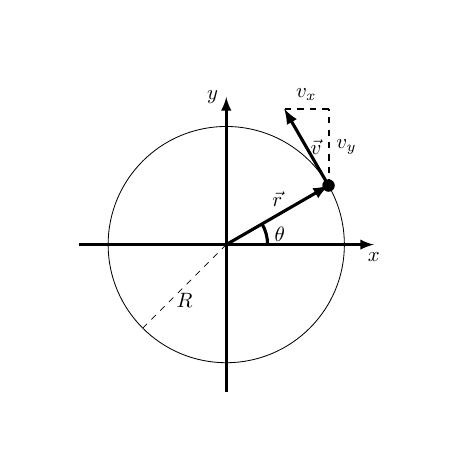
\begin{tikzpicture}[scale=1]
\tikzmath{
\R=2;
\th=30;
\Px=\R*cos(\th);
\Py=\R*sin(\th);
\v=1.5;
\vx=-\v*sin(\th);
\vy=\v*cos(\th);
}
\scalebox{0.75}{

\coordinate (P) at (\Px,\Py);

\draw[-latex, line width=1.25pt] (-1.25*\R,0) -- (1.25*\R,0) node[below]{$x$}; 
\draw[-latex, line width=1.25pt] (0,-1.25*\R) -- (0,1.25*\R) node[left]{$y$};

\draw (0,0) circle (\R); 
\fill (P) circle(3pt);
\draw[-latex, line width = 1.5] (0,0) -- (P) node[midway,above] {$\vec r$};
\draw[line width = 1.5] (0.7,0) arc (0:\th:0.7) node[midway,right]{$\theta$};
\draw[-latex, line width = 1.5] (P) -- +(\vx,\vy) node[midway,right=-2pt] {$\vec v$};
\draw[dashed, line width = 1.] (P) -- +(0,\vy) node[midway,right] {$v_y$};
\draw[dashed, line width = 1.] ($(P) +(0,\vy)$) -- +(\vx,0) node[midway,above] {$v_x$};

\draw[dashed] (0,0) --+(225:\R) node[midway,below]{$R$};

}
\end{tikzpicture}
\end{center}
}
\end{frame}


%%%%%%%%%%%%%%%%%%%%%%%%%%%%%%%%
\begin{frame}{Finally}
\begin{itemize}
\item The acceleration vector is given by:
\begin{align*}
\vec a = \textcolor{blue}{a_s \hat v (t)}+ \textcolor{myred}{v(t)\omega \begin{pmatrix}
-\cos\left(\theta(t)\right)\\
-\sin\left(\theta(t)\right)\end{pmatrix}}=\textcolor{blue}{\alpha(t) R\hat v (t)}+ \textcolor{myred}{\omega^2(t) R \begin{pmatrix}
-\cos\left(\theta(t)\right)\\
-\sin\left(\theta(t)\right)\end{pmatrix}}
\end{align*}
where we used the relations $v(t)=\omega(t) R$ and $a_s(t)=\alpha(t) R$.
\item It has two components:
\begin{enumerate}
\item A \textcolor{blue}{component \textbf{tangent to the circle} (parallel to velocity)}, \textbf{if the speed changes} (``tangential'' acceleration), with magnitude:
\begin{align*}
a_s=a_\parallel=a_T=\frac{dv}{dt}=R\alpha
\end{align*}
\item A \textcolor{myred}{component \textbf{towards the center of the circle} (perpendicular to velocity)} \textbf{because the velocity changes direction} (``centripetal'' or ``radial'' acceleration), with magnitude:
\begin{align*}
a_c=a_\perp=a_R=\omega^2 R=\frac{v^2}{R}
\end{align*}
\end{enumerate}
\end{itemize}
\end{frame}


%%%%%%%%%%%%%%%%%%%%%%%%%%%%%%%%



%%%%%%%%%%%%%%%%%%%%%%%%%%%%%%%%



%%%%%%%%%%%%%%%%%%%%%%%%%%%%%%%%



%%%%%%%%%%%%%%%%%%%%%%%%%%%%%%%%



%%%%%%%%%%%%%%%%%%%%%%%%%%%%%%%%



%%%%%%%%%%%%%%%%%%%%%%%%%%%%%%%%





%%%%%%%%%%%%%%%%%%%%%%%%%%%%%%%%



%%%%%%%%%%%%%%%%%%%%%%%%%%%%%%%%



%%%%%%%%%%%%%%%%%%%%%%%%%%%%%%%%



%%%%%%%%%%%%%%%%%%%%%%%%%%%%%%%%



%%%%%%%%%%%%%%%%%%%%%%%%%%%%%%%%



%%%%%%%%%%%%%%%%%%%%%%%%%%%%%%%%



%%%%%%%%%%%%%%%%%%%%%%%%%%%%%%%%



%%%%%%%%%%%%%%%%%%%%%%%%%%%%%%%%



%%%%%%%%%%%%%%%%%%%%%%%%%%%%%%%%



%%%%%%%%%%%%%%%%%%%%%%%%%%%%%%%%



%%%%%%%%%%%%%%%%%%%%%%%%%%%%%%%%



%%%%%%%%%%%%%%%%%%%%%%%%%%%%%%%%



%%%%%%%%%%%%%%%%%%%%%%%%%%%%%%%%






\end{document}


